\documentclass[a4paper,titlepage]{article}

\usepackage{fullpage}
\usepackage{fontenc}
\usepackage{mathptmx}
\usepackage{xcolor}
\usepackage{tikz}
\usepackage{graphicx}
\usepackage{float}
\usepackage{parskip}

\title{Conversión de ATM a GUI}
\author{Mauro Ezequiel Moltrasio}
\date{}

\begin{document}

\maketitle

El enunciado provisto para el ejercicio sólo requiere la creación de una GUI,
por lo que se eligió modificar el ejercicio de códificación de ATM para que
utilice una interfaz basada en JavaFX. Como primer paso, se simplificaron los
casos de uso para que sean sólo 4:

\begin{figure}[H]
    \centering
    \scalebox{.75}{
        \input{build/uml.tex}
    }
\end{figure}

Teniendo 4 casos de uso para implementar, resulta fácil plantear un escenario
en el que se utilizará un TextArea como pantalla del ATM y 4 botones para la
interacción con el usuario. La pantalla en cuestión tendrá el siguiente
aspecto:

\begin{figure}[H]
    \centering
    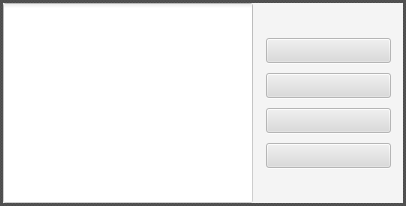
\includegraphics[scale=0.5]{imgs/atm-fxml.png}
\end{figure}

Con el propósito de poder reutilizar la misma escena para los distintos casos,
se implementaron métodos en la clase ATM que modifican los manejadores de
evento de cada botón. De esta manera, en el menú principal cada botón tiene
la funcionalidad necesaria para cambiar el cajero a otro estado (por ejemplo,
al estado crear cuenta) y como parte de este cambio de estado también se altera
la funcionalidad de cada botón. Adicionalmente, para el ingreso de montos
necesario en algunos estados se implementó un manejador de evento para teclas
tipeadas que se agrega al evento onKeyTyped del contenedor de la aplicación.

El diagrama de clases actualizado de la aplicación se adjunta a continuación,
vemos que la mayor parte de métodos de la clase ATM son privados, ya que se
llaman directamente desde manejadores de la misma clase.

\begin{figure}[H]
    \centering
    \scalebox{.5}{
        \input{build/uml_001.tex}
    }
\end{figure}

\end{document}
